\documentclass[notes,11pt, aspectratio=169, xcolor=table]{beamer}

\usepackage{pgfpages}
% These slides also contain speaker notes. You can print just the slides,
% just the notes, or both, depending on the setting below. Comment out the want
% you want.
\setbeameroption{hide notes} % Only slide
%\setbeameroption{show only notes} % Only notes
%\setbeameroption{show notes on second screen=right} % Both

\usepackage{helvet}
\usepackage[default]{lato}
\usepackage{array}

\newtheorem{proposition}{Proposition}
\newcommand{\blue}[1]{\textcolor{blue}{#1}}

\usepackage{tikz}
\usetikzlibrary{shapes.geometric}
\usepackage{pgfplots}
\usetikzlibrary{patterns, pgfplots.fillbetween}
\usepackage{graphicx}
\usepackage{verbatim}
\setbeamertemplate{note page}{\pagecolor{yellow!5}\insertnote}
\usetikzlibrary{positioning}
\usetikzlibrary{snakes}
\usetikzlibrary{calc}
\usetikzlibrary{arrows}
\usetikzlibrary{decorations.markings}
\usetikzlibrary{shapes.misc}
\usetikzlibrary{matrix,shapes,arrows,fit,tikzmark}
\usepackage{amsmath}
\usepackage{mathpazo}
\usepackage{hyperref}
\usepackage{lipsum}
\usepackage{multimedia}
\usepackage{graphicx}
\usepackage{multirow}
\usepackage{graphicx}
\usepackage{dcolumn}
\usepackage{bbm}
\usepackage[style=authoryear,sorting=nyt,uniquename=false]{biblatex}

\addbibresource{references.bib} 

\newcolumntype{d}[0]{D{.}{.}{5}}

\def\@@mybluebox[#1][#2]#3{
    \sbox\mytempbox{#3}%
    \mytemplen\ht\mytempbox
    \advance\mytemplen #1\relax
    \ht\mytempbox\mytemplen
    \mytemplen\dp\mytempbox
    \advance\mytemplen #2\relax
    \dp\mytempbox\mytemplen
    \colorbox{myblue}{\hspace{1em}\usebox{\mytempbox}\hspace{1em}}}


\usepackage{changepage}
\usepackage{appendixnumberbeamer}
\newcommand{\beginbackup}{
   \newcounter{framenumbervorappendix}
   \setcounter{framenumbervorappendix}{\value{framenumber}}
   \setbeamertemplate{footline}
   {
     \leavevmode%
     \hline
     box{%
       \begin{beamercolorbox}[wd=\paperwidth,ht=2.25ex,dp=1ex,right]{footlinecolor}%
%         \insertframenumber  \hspace*{2ex} 
       \end{beamercolorbox}}%
     \vskip0pt%
   }
 }
\newcommand{\backupend}{
   \addtocounter{framenumbervorappendix}{-\value{framenumber}}
   \addtocounter{framenumber}{\value{framenumbervorappendix}} 
}


\usepackage{graphicx}
\usepackage[space]{grffile}
\usepackage{booktabs}

% These are my colors -- there are many like them, but these ones are mine.
\definecolor{blue}{RGB}{0,114,178}
\definecolor{red}{RGB}{213,94,0}
\definecolor{yellow}{RGB}{240,228,66}
\definecolor{green}{RGB}{0,158,115}
\newcommand{\blue}[1]{\textcolor{blue}{#1}}

\hypersetup{
  colorlinks=false,
  linkbordercolor = {white},
  linkcolor = {blue}
}


%% I use a beige off white for my background
\definecolor{MyBackground}{RGB}{255,253,218}

%% Uncomment this if you want to change the background color to something else
%\setbeamercolor{background canvas}{bg=MyBackground}

%% Change the bg color to adjust your transition slide background color!
\newenvironment{transitionframe}{
  \setbeamercolor{background canvas}{bg=yellow}
  \begin{frame}}{
    \end{frame}
}

\setbeamercolor{frametitle}{fg=blue}
\setbeamercolor{title}{fg=blue}
\setbeamertemplate{footline}[frame number]
\setbeamertemplate{navigation symbols}{} 
\setbeamertemplate{itemize items}{-}
\setbeamercolor{itemize item}{fg=blue}
\setbeamercolor{itemize subitem}{fg=blue}
\setbeamercolor{enumerate item}{fg=blue}
\setbeamercolor{enumerate subitem}{fg=blue}
\setbeamercolor{button}{bg=MyBackground,fg=blue,}



% If you like road maps, rather than having clutter at the top, have a roadmap show up at the end of each section 
% (and after your introduction)
% Uncomment this is if you want the roadmap!
% \AtBeginSection[]
% {
%    \begin{frame}
%        \frametitle{Roadmap of Talk}
%        \tableofcontents[currentsection]
%    \end{frame}
% }
\setbeamercolor{section in toc}{fg=blue}
\setbeamercolor{subsection in toc}{fg=red}
\setbeamersize{text margin left=1em,text margin right=1em} 

\newenvironment{wideitemize}{\itemize\addtolength{\itemsep}{10pt}}{\enditemize}

\usepackage{environ}
\NewEnviron{videoframe}[1]{
  \begin{frame}
    \vspace{-8pt}
    \begin{columns}[onlytextwidth, T] % align columns
      \begin{column}{.58\textwidth}
        \begin{minipage}[t][\textheight][t]
          {\dimexpr\textwidth}
          \vspace{8pt}
          \hspace{4pt} {\Large \sc \textcolor{blue}{#1}}
          \vspace{8pt}
          
          \BODY
        \end{minipage}
      \end{column}%
      \hfill%
      \begin{column}{.42\textwidth}
        \colorbox{green!20}{\begin{minipage}[t][1.2\textheight][t]
            {\dimexpr\textwidth}
            Face goes here
          \end{minipage}}
      \end{column}%
    \end{columns}
  \end{frame}
}

\title[]{International Trade: Lecture 2}
\subtitle[]{Intro to Classical Ricardian Trade}
\author[Góes]
{Carlos Góes\inst{1}}
\date{Fall 2025}
\institute[GWU]{\inst{1} George Washington University }



\begin{document}

%%% TIKZ STUFF
\tikzset{   
        every picture/.style={remember picture,baseline},
        every node/.style={anchor=base,align=center,outer sep=1.5pt},
        every path/.style={thick},
        }
\newcommand\marktopleft[1]{%
    \tikz[overlay,remember picture] 
        \node (marker-#1-a) at (-.3em,.3em) {};%
}
\newcommand\markbottomright[2]{%
    \tikz[overlay,remember picture] 
        \node (marker-#1-b) at (0em,0em) {};%
}
\tikzstyle{every picture}+=[remember picture] 
\tikzstyle{mybox} =[draw=black, very thick, rectangle, inner sep=10pt, inner ysep=20pt]
\tikzstyle{fancytitle} =[draw=black,fill=red, text=white]
%%%% END TIKZ STUFF



%----------------------------------------------------------------------%
%-------------------       TITLE PAGE       ---------------------------%
%----------------------------------------------------------------------%





%----------------------------------------------------------------------%






%----------------------------------------------------------------------%
%----------------------------------------------------------------------%

%----------------------------------------------------------------------%
\frame{\titlepage}
\addtocounter{framenumber}{-1}
%----------------------------------------------------------------------%



%----------------------------------------------------------------------%
%----------------------------------------------------------------------%


\begin{frame}{David Ricardo (1772–1823)}
\begin{columns}
    \begin{column}{0.65\textwidth}
        \begin{wideitemize}
            \item Born: April 18, 1772, London (third of 17 children)
            \item Career: Achieved wealth through disciplined financial trading in government consols and loans
            \item Major Work: \textit{On the Principles of Political Economy and Taxation} (1817) – foundational text on comparative advantage, value, rent, etc.
            \item Public Life: MP for Portarlington (1819–1823), promoting free trade, currency reform, and abolition
            \item Death: Died Sept. 11, 1823, age 51, from septic ear infection
        \end{wideitemize}
    \end{column}
    
    \begin{column}{0.35\textwidth}
        \centering
        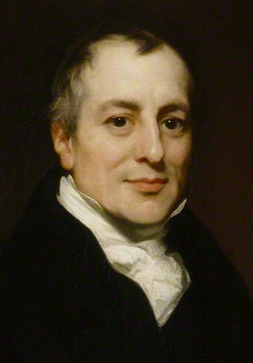
\includegraphics[width=\linewidth]{figs/ricardo.jpg} % Replace with your image filename
        \vspace{0.2cm}
        \scriptsize\textit{David Ricardo (public domain image)}
    \end{column}
\end{columns}
\end{frame}

\begin{frame}{Mathematical Preliminaries}

\begin{wideitemize}
    \item A set is an unordered collection of distinct objects, also known as elements.
    \item<2-> Suppose $\mathcal{N}$ is the set of neighborhoods in Washington, DC. We write:
    \begin{equation*}
        \mathcal{N} = \{ \text{Foggy Bottom}, \text{Navy Yard}, \text{Anacostia}, \text{Noma}, \text{Union Market}, \text{Capitol Hill}, \cdots \}
    \end{equation*}

    \item<3-> Let $\mathcal{N}^{NW}$ be the set of neighborhoods in Northwest DC:
    \begin{equation*}
        \mathcal{N}^{NW} = \{ \text{Foggy Bottom}, \text{West End}, \text{Dupont Circle}, \text{Logan Circle}, \text{Shaw}, \cdots \}  
    \end{equation*}
          

    \item<4-> We say that \blue{$\mathcal{N}^{NW}$ is a subset of $\mathcal{N}$} and write $\mathcal{N}^{NW} \subset \mathcal{N}$
\end{wideitemize}
    
\end{frame}

\begin{frame}{Fixed costs and increasing returns}
\normalsize

\begin{columns}[T] % align columns
\begin{column}{.45\textwidth}
            \centering
\begin{tikzpicture}[x=\textwidth/60, y=\textwidth/60] % 2:1 aspect
  \draw[very thick] ( 0,0) ellipse (27 and 27);
  \draw[very thick] (  0,0) ellipse (21 and 21);
  \draw[very thick] ( 0,0) ellipse (15 and  15);
  \draw[very thick] (0,0) ellipse ( 9 and  9);

  \node[font=\bfseries\Large] at (0,0) {$\mathbb{N}$};
  \node[font=\bfseries\Large] at ( 0,10) {$\mathbb{Z}$};
  \node[font=\bfseries\Large] at (  0,16) {$\mathbb{Q}$};
  \node[font=\bfseries\Large] at ( 0,22) {$\mathbb{R}$};
\end{tikzpicture}
    

                
    \end{column}
    \begin{column}{.45\textwidth}

    \begin{wideitemize}
        \item \blue{Another example}: natural numbers are a subset of integers, which is a subset of the rationals, which is a subset of the real numbers.
        \item<2-> How can we denote the set of natural numbers (strictly) smaller than 10?

        \item<3-> Like this:

        \begin{equation*}
            \left\{ x \in \mathbb{N} : 0 \le x < 10 \right\}
        \end{equation*}
    \end{wideitemize}



\end{column}
\end{columns}


\end{frame}



\begin{frame}{Ricardian Model: Preliminaries}
\begin{wideitemize}
        \item Consider a world with 2 countries (US, Colombia) and 2 products (Computers, Roses)
        \item<2-> Set of countries $i \in \{ US, COL\}$; set of products $p \in \{ C, R\}$
        \item<3-> In country $i$, there are $L_i$ units of labor (worker-hours) available 
        \item<4-> In country $i$, to produce one unit of good $p$, firms use $a_{i,p}$ units of labor
        \item<5-> $Y_{i,p}$ is total production of good $p$ in $i$
        \item<6-> To produce $Y_{i,C}$ units of computers in $i$, firms use $a_{i,C} \times Y_{i,C}$ units of labor 
        \item<6-> We call $a_{i,p}$ the \textbf{unit labor requirements}
        \begin{itemize}
            \item<6-> The higher $a_{i,p}$, the \textbf{less productive} country $i$ is in producing $p$. Why?
        \end{itemize}
        \item<7-> Trade is balanced
    \end{wideitemize}
\end{frame}

\section{Production}

\begin{frame}{Production Possibilities Frontier}
\begin{wideitemize}
        \item Total labor can be distributed for the production of either good, such that:

        \begin{equation*}
            \underbrace{a_{i,C} \times Y_{i,C}}_{\substack{\text{labor used in} \\ \text{production of } C}} + \underbrace{a_{i,R} \times Y_{i,R}}_{\substack{\text{labor used in} \\ \text{production of } R}} \le \underbrace{L_i}_{\substack{\text{total labor} \\ \text{available in } i}}
        \end{equation*}

        \item<2-> Inequality above defines set of feasible production choices, formally:

        \begin{equation*}
            \mathcal{Y}_{i} = \{ (Y_{i,C}, Y_{i,R}) : a_{i,C} \times Y_{i,C} + a_{i,R} \times Y_{i,R} \le L_i \}
        \end{equation*}
        
        \item<2-> English: if labor used to produce $(Y_{i,C}, Y_{i,R})$ is not larger than $L_i$, production is feasible
    \end{wideitemize}
\end{frame}

\begin{frame}{Production Possibilities Frontier, Example}
\begin{wideitemize}
        \item There are 300 million units of labor in the US ($L_{US} = 300$ million)
        \item<2-> To produce one rose in the US, firms use $30$ units of labor ($a_{US,R} = 30$)
        \item<3-> To produce one computer in the US, firms use $3,000$ units of labor ($a_{US,C} = 3,000$)
        \item<4-> How many units of either good can the US make?
        \begin{itemize}
            \item<4-> If it fully specializes in $R$, it can produce $Y_{US,R}=L_{US}/a_{US,R} = 300 \text{ million}/30 = 10 \text{ million}$ roses.
            \item<4-> If it fully specializes in $C$, it can produce $Y_{US,C}=L_{US}/a_{US,C} = 300 \text{ million}/3,000 = 100,000$ computers.
        \end{itemize}

        \item<5-> In general, it can produce any combination $(Y_{US,R}, Y_{US,C})$ that satisfies:

        \begin{equation*}
            3,000 \times Y_{US,C} + 30 \times Y_{US,R} \le 300 \text{ million}
        \end{equation*}
    \item<6-> Opportunity cost: $a_{US,R}/a_{US,C} = 30/3000 = 1/100$ computers per rose \\
    \qquad \textcolor{gray}{(or $a_{US,C}/a_{US,R} = 100$ roses per computer)}
    \end{wideitemize}
\end{frame}

\begin{frame}{Production Possibilities Frontier, Graphical Example}

\begin{center}

\begin{figure}[htbp]

\begin{tikzpicture}
\begin{axis}[
    xlabel={Quantity of roses, $Y_{US,R}$},
    ylabel={Quantity of computers, $Y_{US,C}$},
    xmin=0, xmax=11,
    ymin=0, ymax=0.11,
    yticklabel=\empty,
    xticklabel=\empty,
    axis lines=left,
    enlargelimits=false,
    clip=false,
    axis on top,
    scaled x ticks=false,
    width=9cm, height=7cm,
    title={US},
    title style={font=\bfseries}
]

% Filled triangle under the PPF
\addplot [
    name path=A,
    domain=0:0.1,
    draw=none
] {.1 - 1/100*x};

\path[name path=B] (axis cs:0,0) -- (axis cs:10,0);

\addplot [
    fill=cyan!20,
    draw=none
] fill between [of=A and B];

% PPF line
\addplot[thick, blue, domain=0:10] {.1 - 1/100*x};

% Labels
\node at (axis cs:3.5,0.03) {\Large $\mathcal{Y}_{US}$};
\node at (axis cs:10,-.01) {\scriptsize $\frac{L_{US}}{a_{US,R}}$};
\node at (axis cs:-.75,.1) {\scriptsize $\frac{L_{US}}{a_{US,C}}$};
\node at (axis cs:10,0.05) { $\textcolor{blue}{Y_{US,C} = \frac{L_{US}}{a_{US,C}} - \frac{a_{US,R}}{a_{US,C}} \times Y_{US,R}}$};
\node at (axis cs:7,0.07) {\scriptsize \textcolor{blue}{Slope = - 1/100: opportunity cost} };

\end{axis}

\end{tikzpicture}

\end{figure}
\end{center}


\end{frame}


\begin{frame}{Production Technology}
\begin{wideitemize}
        \item In country $i$, firms producing good $p$ maximize profits under perfect competition:
        \begin{equation*}
            \max_{Y_{i,p}} \pi_{i,p} = \max_{Y_{i,p}} P_{i,p}Y_{i,p} - w_i a_{i,p} Y_{i,p} 
        \end{equation*}
        \item<2-> Since labor only one type of labor (mobile across sectors), there is a single wage $w_i$
        \item<3-> In equilibrium, \textbf{prices equal marginal cost} in each productive sector:
        \begin{eqnarray*}
            P_{i,p} = w_i a_{i,p} \iff \frac{P_{i,p}}{a_{i,p}} = w_i  \qquad \text{ for } p \in\{C,R\}
        \end{eqnarray*}
        \item<4-> In autarky equilibrium, there demand and production in both sectors
        \item<5-> We can pin down the relative price $P_{i,C} / P_{i,R}$:
        \begin{equation*}
            \frac{P_{i,C}}{a_{i,C}} = w_i = \frac{P_{i,R}}{a_{i,R}} \iff \frac{P_{i,C}}{P_{i,R}} = \frac{a_{i,C}}{a_{i,R}}  
        \end{equation*}
    \item<6-> In autarky, relative prices will reflect the \textbf{opportunity cost} within country $i$
    \end{wideitemize}
\end{frame}


\begin{frame}{Production Possibilities Frontier, Graphical Example}

\begin{center}

\begin{figure}[htbp]

\begin{tikzpicture}

\begin{axis}[
    xlabel={Quantity of roses, $Y_{US,R}$},
    ylabel={Quantity of computers, $Y_{US,C}$},
    xmin=0, xmax=11,
    ymin=0, ymax=0.11,
    yticklabel=\empty,
    xticklabel=\empty,
    axis lines=left,
    enlargelimits=false,
    clip=false,
    axis on top,
    scaled x ticks=false,
    width=9cm, height=7cm,
    title={US},
    title style={font=\bfseries}
]

% Filled triangle under the PPF
\addplot [
    name path=A,
    domain=0:0.1,
    draw=none
] {.1 - 1/100*x};

\path[name path=B] (axis cs:0,0) -- (axis cs:10,0);

\addplot [
    fill=cyan!20,
    draw=none
] fill between [of=A and B];

% PPF line
\addplot[thick, blue, domain=0:10] {.1 - 1/100*x};

% Labels
\node at (axis cs:3.5,0.03) {\Large $\mathcal{Y}_{US}$};
\node at (axis cs:10,-.01) {\scriptsize $\frac{L_{US}}{a_{US,R}}$};
\node at (axis cs:-.75,.1) {\scriptsize $\frac{L_{US}}{a_{US,C}}$};
\node at (axis cs:10,0.05) { $\textcolor{blue}{Y_{US,C} = \frac{L_{US}}{a_{US,C}} -} \textcolor{red}{ \frac{P_{US,R}}{P_{US,C}} } \textcolor{blue}{ \times Y_{US,R}}$};
\node at (axis cs:10,0.07) {\scriptsize \textcolor{red}{Slope = - 1/100: opportunity cost = relative prices} };



\end{axis}

\end{tikzpicture}

\end{figure}
\end{center}


\end{frame}

\section{Preferences}

\begin{frame}{Preferences}
\begin{wideitemize}
        \item In country $i$, consumers preferences over products $p$, represented by a utility function:
        \begin{equation*}
            U_i(Q_C,Q_R) \equiv Q_C^{\alpha_i} Q_R^{1-\alpha_i}, \qquad \text{for } 0 < \alpha_i < 1   
        \end{equation*}
        \item<2-> We call these \textbf{Cobb-Douglas Preferences}
        \item<3-> Some characteristics:
        \begin{itemize}
            \item<3-> Increasing in both arguments \\
            \qquad \qquad \textcolor{gray}{(happier if consume more $Q_C$ or $Q_R$)}

            \begin{equation*}
                \frac{\partial U_i(Q_C,Q_R)}{\partial Q_C} > 0, \qquad \frac{\partial U_i(Q_C,Q_R)}{\partial Q_R} > 0
            \end{equation*}
            \item<4-> Marginal decreasing utility \\
            \qquad \qquad \textcolor{gray}{(lower increase for each additional $Q_C$, holding $Q_R$ fixed)}
            \begin{eqnarray*}
                \frac{\partial}{\partial Q_C} \left[ \frac{\partial U_i(Q_C,Q_R)}{\partial Q_C} \right] = \frac{\partial^2 U_i(Q_C,Q_R)}{\partial Q_C^2} &<& 0, \\
                \qquad \frac{\partial}{\partial Q_R} \left[ \frac{\partial U_i(Q_C,Q_R)}{\partial Q_R} \right] = \frac{\partial^2 U_i(Q_C,Q_R)}{\partial Q_R^2} &<& 0
            \end{eqnarray*}
            
        \end{itemize}
    \end{wideitemize}
\end{frame}


\begin{frame}{Preferences}
\begin{wideitemize}
        \item In country $i$, consumers preferences over products $p$, represented by a utility function:
        \begin{equation*}
            U_i(Q_C,Q_R) \equiv Q_C^{\alpha_i} Q_R^{1-\alpha_i}, \qquad \text{for } 0 < \alpha_i < 1   
        \end{equation*}
        \item How to derive indifference curves?
        \begin{eqnarray*}
            U_i = Q_C^{\alpha_i} Q_R^{1-\alpha_i} \iff Q_C^{\alpha_i} = U_i \times Q_R^{-(1-\alpha_i)} \iff Q_C = U_i^{\frac{1}{\alpha_i}} \times Q_R^{-\frac{1-\alpha_i}{\alpha_i}} 
        \end{eqnarray*}
        \item<2-> Example: Suppose $\alpha_i=1/2$. Then:
        \begin{equation*}
            Q_C = U_i^{\frac{1}{1/2}} \times Q_R^{-\frac{1-1/2}{1/2}} = U_i^{2} \times Q_R^{-1} = \frac{U_i^{2}}{Q_R} 
        \end{equation*}
        \item<3-> English: for fixed utility $U_i$, if consumption $Q_R$ goes up, consumption $Q_C$ must go down
    \end{wideitemize}
\end{frame}



\begin{frame}{Preferences, Graphically}

\begin{figure}[htbp]

\begin{tikzpicture}


\begin{axis}[
    xlabel={Quantity of computers, $Q_{C}$},
    ylabel={Quantity of roses, $Q_{R}$},
    xmin=0, xmax=0.11,
    ymin=0, ymax=21,
    yticklabel=\empty,
    xticklabel=\empty,
    axis lines=left,
    enlargelimits=false,
    clip=false,
    axis on top,
    scaled x ticks=false,
    width=9cm, height=7cm,
    title style={font=\bfseries}
]

% PPF line
\addplot[black, domain=0.01:0.1] {0.1 / x};
\addplot[blue, domain=0.0125:0.1] {0.2 / x};
\addplot[red, domain=0.015:0.1] {0.3 / x};


\end{axis}

\end{tikzpicture}

\end{figure}

\end{frame}

\section{Autarky Equilibrium}

\begin{frame}{Ricardian Model: Autarky Equilibrium}


\begin{wideitemize}
    \item In equilibrium, relative prices = marginal rate of substitution. Why? \\
    \qquad \textcolor{gray}{(check handout for math; we will solve the full problem next lecture)}

    \item<2-> \textcolor{blue}{Relative prices} $P_{i,R}/P_{i,C}$: marginal cost of replacing roses for computers

    \item<3-> \textcolor{blue}{Marginal rate of substitution} $MU_{i,R}/MU_{i,C}$: marginal benefit of of replacing roses for computers

    \begin{equation*}
        MRS_{i,R,C} = \frac{MU_{i,R}}{MU_{i,C}} = \frac{ \partial U_i / \partial Q_R }{\partial U_i / \partial Q_C  } = \frac{ (1-\alpha_i ) Q_C^{\alpha_i} Q_R^{1-\alpha_i} Q_{R}^{-1} }{ \alpha_i  Q_C^{\alpha_i} Q_R^{1-\alpha_i} Q_{C}^{-1} } = \frac{1-\alpha_i}{\alpha_i} \times \frac{Q_C}{Q_R}
    \end{equation*}


    \item<4-> English (sort of): marginal cost = marginal benefit 
    \end{wideitemize}

\end{frame}

\begin{frame}{Autarky Equilibrium, Graphical Example}

\pgfmathsetmacro{\aC}{100}       % unit labor requirement for computers
\pgfmathsetmacro{\aR}{1}         % unit labor requirement for roses
\pgfmathsetmacro{\alpha}{0.5}    % preference for computers
\pgfmathsetmacro{\Lendow}{10}    % labor endowment

% Compute equilibrium quantities
\pgfmathsetmacro{\Qc}{(\alpha*\Lendow)/\aC}
\pgfmathsetmacro{\Qr}{((1 - \alpha)*\Lendow)/\aR}

% Compute utility level
\pgfmathsetmacro{\U}{(\Qc^(\alpha))*(\Qr^(1 - \alpha))}

% Compute prefactor for indifference curve: Qc = A * Qr^(- (1 - alpha)/alpha)
\pgfmathsetmacro{\expo}{(1 - \alpha)/\alpha}
\pgfmathsetmacro{\A}{\U^(1/\alpha)}

\begin{center}
\begin{figure}[htbp]
\centering
\begin{tikzpicture}
\begin{axis}[
    ylabel={Quantity of computers, $\textcolor{red}{Q_{US,C}}, \textcolor{blue}{Y_{US,C}}$},
    xlabel={Quantity of roses, $\textcolor{red}{Q_{US,R}}, \textcolor{blue}{Y_{US,R}}$},
    ymin=0, ymax=0.11,
    xmin=0, xmax=11,
    yticklabel=\empty,
    xticklabel=\empty,
    axis lines=left,
    enlargelimits=false,
    clip=false,
    axis on top,
    scaled x ticks=false,
    width=9cm, height=7cm,
    title style={font=\bfseries}
]

% PPF: Q_C = (L/a_C) - (a_R/a_C) * Q_R
\addplot[thick, blue, domain=0:10] {\Lendow/\aC - (\aR/\aC)*x};

% Indifference curve through optimal bundle
\addplot[red, domain=2.5:10, samples=100] {\A * x^(-\expo)};

% Fill under the PPF
\addplot [
    name path=ppfcurve,
    domain=0:10,
    draw=nonC
] {\Lendow/\aC - (\aR/\aC)*x};

\addplot [
    name path=xaxis,
    domain=0:0.1,
    draw=none
] {0};

\addplot [
    fill=cyan!20,
    draw=none
] fill between [of=ppfcurve and xaxis];

% Labels

%\node at (axis cs:3.5,0.03) {\Large $\mathcal{Y}_{US}$};
\node at (axis cs:\Lendow/\aR,-.01) {\scriptsize $\frac{L_{US}}{a_{US,R}}$};
\node at (axis cs:-.75,\Lendow/\aC) {\scriptsize $\frac{L_{US}}{a_{US,C}}$};


% Equilibrium point
\addplot[only marks, mark=*, color=red, mark size=2pt] coordinates {(\Qr, \Qc)};
\node at (axis cs:\Qr - 1,\Qc - 0.01) {\scriptsize $\frac{P_{US,R}}{P_{US,C}} = MRS_{US,R,C}$};
\node at (axis cs:\Qr + 1.25,\Qc + 0.005) {\scriptsize $\textcolor{red}{(Q_{US,R},Q_{US,C})}$};

\end{axis}
\end{tikzpicture}
\end{figure}
\end{center}

\end{frame}


\begin{frame}{What about Colombia?}
\begin{wideitemize}
        \item There are 54 million units of labor in Colombia ($L_{COL} = 54$ million)
        \item<2-> To produce one rose in Colombia, firms use $6$ units of labor ($a_{COL,R} = 6$)
        \item<3-> To produce one computer in Colombia, firms use $5,400$ units of labor ($a_{COL,C} = 5,400$)
        \item<4-> How many units of either good can Colombia make?
        \begin{itemize}
            \item<4-> If it fully specializes in $R$, it can produce $Y_{COL,R}=L_{COL}/a_{COL,R} = 54 \text{ million}/6 = 9 \text{ million}$ roses.
            \item<4-> If it fully specializes in $C$, it can produce $Y_{COL,C}=L_{COL}/a_{COL,C} = 54 \text{ million}/5,400 = 10,000$ computers.
        \end{itemize}

        \item<5-> In general, it can produce any combination $(Y_{COL,R}, Y_{COL,C})$ that satisfies:

        \begin{equation*}
            5,400 \times Y_{COL,C} + 6 \times Y_{COL,R} \le 54 \text{ million}
        \end{equation*}
        \item<6-> Opportunity cost: $a_{COL,R} / a_{COL,C} = 6 / 5,400 = 1/900$. \\
        \qquad \textcolor{gray}{(this will also be the equal to relative prices!)}
    \end{wideitemize}
\end{frame}


\begin{frame}{Autarky Equilibrium, Colombia}

\pgfmathsetmacro{\aC}{900}       % unit labor requirement for computers
\pgfmathsetmacro{\aR}{1}         % unit labor requirement for roses
\pgfmathsetmacro{\alpha}{0.75}    % preference for computers
\pgfmathsetmacro{\Lendow}{9}    % labor endowment

% Compute equilibrium quantities
\pgfmathsetmacro{\Qc}{(\alpha*\Lendow)/\aC}
\pgfmathsetmacro{\Qr}{((1 - \alpha)*\Lendow)/\aR}

% Compute utility level
\pgfmathsetmacro{\U}{(\Qc^(\alpha))*(\Qr^(1 - \alpha))}

% Compute prefactor for indifference curve: Qc = A * Qr^(- (1 - alpha)/alpha)
\pgfmathsetmacro{\expo}{(1 - \alpha)/\alpha}
\pgfmathsetmacro{\A}{\U^(1/\alpha)}

\begin{center}
\begin{figure}[htbp]
\centering
\begin{tikzpicture}
\begin{axis}[
    ylabel={Quantity of computers, $\textcolor{red}{Q_{COL,C}}, \textcolor{blue}{Y_{COL,C}}$},
    xlabel={Quantity of roses, $\textcolor{red}{Q_{COL,R}}, \textcolor{blue}{Y_{COL,R}}$},
    ymin=0, ymax=0.11,
    xmin=0, xmax=11,
    yticklabel=\empty,
    xticklabel=\empty,
    axis lines=left,
    enlargelimits=false,
    clip=false,
    axis on top,
    scaled x ticks=false,
    width=9cm, height=7cm,
    title style={font=\bfseries}
]

% PPF: Q_C = (L/a_C) - (a_R/a_C) * Q_R
\addplot[thick, blue, domain=0:9] {\Lendow/\aC - (\aR/\aC)*x};

% Indifference curve through optimal bundle
\addplot[red, domain=0.1:9, samples=100] {\A * x^(-\expo)};

% Fill under the PPF
\addplot [
    name path=ppfcurve,
    domain=0:9,
    draw=nonC
] {\Lendow/\aC - (\aR/\aC)*x};

\addplot [
    name path=xaxis,
    domain=0:0.1,
    draw=none
] {0};

\addplot [
    fill=cyan!20,
    draw=none
] fill between [of=ppfcurve and xaxis];

% Labels

%\node at (axis cs:3.5,0.03) {\Large $\mathcal{Y}_{US}$};
\node at (axis cs:\Lendow/\aR,-.01) {\scriptsize $\frac{L_{COL}}{a_{COL,R}}$};
\node at (axis cs:-.75,\Lendow/\aC) {\scriptsize $\frac{L_{COL}}{a_{COL,C}}$};


% Equilibrium point
\addplot[only marks, mark=*, color=red, mark size=2pt] coordinates {(\Qr, \Qc)};
\node at (axis cs:\Qr + 1.25,\Qc + 0.005) {\scriptsize $\textcolor{red}{(Q_{COL,R},Q_{COL,C})}$};

\end{axis}
\end{tikzpicture}
\end{figure}
\end{center}

\end{frame}


\section{Absolute and Comparative Advantage}

\begin{frame}{Absolute and Comparative Advantage}

\begin{wideitemize}
    \item We say Colombia has an \textcolor{blue}{absolute advantage} in the production of good $p$ if $a_{COL,p} < a_{US,p}$

    \item English: absolute advantage in production = uses less labor to produce one unit \\
    \qquad \textcolor{gray}{(i.e., it is more productive)}

    \item<2-> \textcolor{blue}{Opportunity cost}: cost of producing a good, measured in foregone output of all others.

    \item<2-> \blue{Comparative advantage}: An economy has a comparative advantage in producing a good if its opportunity cost of the good is lower than in the rest of the world.

\end{wideitemize}

\end{frame}


\begin{frame}{Absolute and Comparative Advantage}

\begin{wideitemize}

    \item We say Colombia has an \textcolor{blue}{comparative advantage} in the production of roses, since:
    
    \begin{equation*}
        1/900 = a_{COL,R}/a_{COL,C} < a_{US,R}/a_{US,C} = 1/100
    \end{equation*}

    \item<2-> We say the US has an \textcolor{blue}{comparative advantage} in the production of computers, since:
    
    \begin{equation*}
        900 = a_{COL,C}/a_{COL,R
        } > a_{US,C}/a_{US,R} = 100
    \end{equation*}

\end{wideitemize}

\end{frame}


\begin{frame}{Comparative Advantage}

\begin{wideitemize}

    \item Without trade, prices reflect opportunity cost:
    \begin{itemize}
        \item In Colombia: $a_{COL,R}/a_{COL,C} = P_{COL,R}/P_{COL,C}$
        \item In the US: $a_{US,R}/a_{US,C} = P_{US,R}/P_{US,C}$
    \end{itemize}

    \item<2-> Under free trade, there are world prices, i.e. $P_R,P_C$ that hold both in countries. Why? \\
        \qquad \textcolor{gray}{(goods are assumed to be identical)}

    \item<3->  In this model, \blue{countries specialize in goods in which they have a comparative advantage} after trade:
    
    \begin{itemize}
        \item<3->  \blue{Colombia} specializes in \blue{roses} if $a_{COL,R}/a_{COL,C} < P_R/P_C$
        \item<3-> The \blue{US} specializes in \blue{computers} if $a_{US,R}/a_{US,C} > P_R/P_C$
    \end{itemize}

\end{wideitemize}

\end{frame}


\begin{frame}{Production Possibilities Frontier in Autarky}
\begin{center}

\begin{figure}[htbp]

% California
\begin{subfigure}{}
\resizebox{0.48\linewidth}{!}{%
\begin{tikzpicture}
\pgfmathsetmacro{\aC}{100}       % unit labor requirement for computers
\pgfmathsetmacro{\aR}{1}         % unit labor requirement for roses
\pgfmathsetmacro{\alpha}{0.5}    % preference for computers
\pgfmathsetmacro{\Lendow}{10}    % labor endowment

% Compute equilibrium quantities
\pgfmathsetmacro{\Qc}{(\alpha*\Lendow)/\aC}
\pgfmathsetmacro{\Qr}{((1 - \alpha)*\Lendow)/\aR}

% Compute utility level
\pgfmathsetmacro{\U}{(\Qc^(\alpha))*(\Qr^(1 - \alpha))}

% Compute prefactor for indifference curve: Qc = A * Qr^(- (1 - alpha)/alpha)
\pgfmathsetmacro{\expo}{(1 - \alpha)/\alpha}
\pgfmathsetmacro{\A}{\U^(1/\alpha)}

\centering
\begin{axis}[
    ylabel={Quantity of computers, $\textcolor{red}{Q_{US,C}}, \textcolor{blue}{Y_{US,C}}$},
    xlabel={Quantity of roses, $\textcolor{red}{Q_{US,R}}, \textcolor{blue}{Y_{US,R}}$},
    ymin=0, ymax=0.11,
    xmin=0, xmax=11,
    yticklabel=\empty,
    xticklabel=\empty,
    axis lines=left,
    enlargelimits=false,
    clip=false,
    axis on top,
    scaled x ticks=false,
    width=9cm, height=7cm,
    title style={font=\bfseries}
]

% PPF: Q_C = (L/a_C) - (a_R/a_C) * Q_R
\addplot[thick, blue, domain=0:10] {\Lendow/\aC - (\aR/\aC)*x};

% Indifference curve through optimal bundle
%\addplot[red, domain=0.1:9, samples=100] {\A * x^(-\expo)};

% Labels

%\node at (axis cs:3.5,0.03) {\Large $\mathcal{Y}_{US}$};
\node at (axis cs:\Lendow/\aR,-.01) {\scriptsize $\frac{L_{US}}{a_{US,R}}$};
\node at (axis cs:-.75,\Lendow/\aC) {\scriptsize $\frac{L_{US}}{a_{US,C}}$};


% Equilibrium point
\addplot[only marks, mark=*, color=blue, mark size=2pt] coordinates {(\Qr, \Qc)};
\node at (axis cs:\Qr - 1.25,\Qc - 0.005) {\scriptsize $\textcolor{blue}{(Q_{US,R},Q_{US,C})}$};
\node at (axis cs:\Qr - 2,\Qc + 0.0025) {\scriptsize $\textcolor{blue}{(Y_{US,R},Y_{US,C})}$};



\end{axis}

\end{tikzpicture}
}
\end{subfigure}
%
% Colombia
\begin{subfigure}{}
\resizebox{0.48\linewidth}{!}{%
\begin{tikzpicture}
\pgfmathsetmacro{\aC}{900}       % unit labor requirement for computers
\pgfmathsetmacro{\aR}{1}         % unit labor requirement for roses
\pgfmathsetmacro{\alpha}{0.75}    % preference for computers
\pgfmathsetmacro{\Lendow}{9}    % labor endowment

% Compute equilibrium quantities
\pgfmathsetmacro{\Qc}{(\alpha*\Lendow)/\aC}
\pgfmathsetmacro{\Qr}{((1 - \alpha)*\Lendow)/\aR}

% Compute utility level
\pgfmathsetmacro{\U}{(\Qc^(\alpha))*(\Qr^(1 - \alpha))}

% Compute prefactor for indifference curve: Qc = A * Qr^(- (1 - alpha)/alpha)
\pgfmathsetmacro{\expo}{(1 - \alpha)/\alpha}
\pgfmathsetmacro{\A}{\U^(1/\alpha)}

\centering
\begin{axis}[
    ylabel={Quantity of computers, $\textcolor{red}{Q_{COL,C}}, \textcolor{blue}{Y_{COL,C}}$},
    xlabel={Quantity of roses, $\textcolor{red}{Q_{COL,R}}, \textcolor{blue}{Y_{COL,R}}$},
    ymin=0, ymax=0.11,
    xmin=0, xmax=11,
    yticklabel=\empty,
    xticklabel=\empty,
    axis lines=left,
    enlargelimits=false,
    clip=false,
    axis on top,
    scaled x ticks=false,
    width=9cm, height=7cm,
    title style={font=\bfseries}
]

% PPF: Q_C = (L/a_C) - (a_R/a_C) * Q_R
\addplot[thick, blue, domain=0:9] {\Lendow/\aC - (\aR/\aC)*x};

% Indifference curve through optimal bundle
%\addplot[red, domain=0.1:9, samples=100] {\A * x^(-\expo)};

% Labels

%\node at (axis cs:3.5,0.03) {\Large $\mathcal{Y}_{US}$};
\node at (axis cs:\Lendow/\aR,-.01) {\scriptsize $\frac{L_{COL}}{a_{COL,R}}$};
\node at (axis cs:-.75,\Lendow/\aC) {\scriptsize $\frac{L_{COL}}{a_{COL,C}}$};


% Equilibrium point
\addplot[only marks, mark=*, color=blue, mark size=2pt] coordinates {(\Qr, \Qc)};
\node at (axis cs:\Qr + 1.25,\Qc + 0.009) {\scriptsize $\textcolor{blue}{(Q_{COL,R},Q_{COL,C})}$};
\node at (axis cs:\Qr + 2.25,\Qc + 0.001) {\scriptsize $\textcolor{blue}{(Y_{COL,R},Y_{COL,C})}$};


\end{axis}

\end{tikzpicture}
}

\end{subfigure}

\caption{Autarky Equilibriun}
\end{figure}
\end{center}
\end{frame}


\begin{frame}{Production Possibilities Frontier + Trade Prices}
\begin{center}

\begin{figure}[htbp]

% California
\begin{subfigure}{}
\resizebox{0.48\linewidth}{!}{%
\begin{tikzpicture}
\pgfmathsetmacro{\aC}{100}       % unit labor requirement for computers
\pgfmathsetmacro{\aR}{1}         % unit labor requirement for roses
\pgfmathsetmacro{\alpha}{0.5}    % preference for computers
\pgfmathsetmacro{\Lendow}{10}    % labor endowment

% Compute equilibrium quantities
\pgfmathsetmacro{\Qc}{(\alpha*\Lendow)/\aC}
\pgfmathsetmacro{\Qr}{((1 - \alpha)*\Lendow)/\aR}

% Compute utility level
\pgfmathsetmacro{\U}{(\Qc^(\alpha))*(\Qr^(1 - \alpha))}

% Compute prefactor for indifference curve: Qc = A * Qr^(- (1 - alpha)/alpha)
\pgfmathsetmacro{\expo}{(1 - \alpha)/\alpha}
\pgfmathsetmacro{\A}{\U^(1/\alpha)}

\centering
\begin{axis}[
    ylabel={Quantity of computers, $\textcolor{red}{Q_{US,C}}, \textcolor{blue}{Y_{US,C}}$},
    xlabel={Quantity of roses, $\textcolor{red}{Q_{US,R}}, \textcolor{blue}{Y_{US,R}}$},
    ymin=0, ymax=0.11,
    xmin=0, xmax=11,
    yticklabel=\empty,
    xticklabel=\empty,
    axis lines=left,
    enlargelimits=false,
    clip=false,
    axis on top,
    scaled x ticks=false,
    width=9cm, height=7cm,
    title style={font=\bfseries}
]

% PPF: Q_C = (L/a_C) - (a_R/a_C) * Q_R
\addplot[thick, blue, domain=0:10] {\Lendow/\aC - (\aR/\aC)*x};

\addplot[thick, red, domain=0:10] {\Lendow/\aC - (1/135)*x};


% Indifference curve through optimal bundle
%\addplot[red, domain=0.1:9, samples=100] {\A * x^(-\expo)};

% Labels

%\node at (axis cs:3.5,0.03) {\Large $\mathcal{Y}_{US}$};
\node at (axis cs:\Lendow/\aR,-.01) {\scriptsize $\frac{L_{US}}{a_{US,R}}$};
\node at (axis cs:-.75,\Lendow/\aC) {\scriptsize $\frac{L_{US}}{a_{US,C}}$};


% Equilibrium point
\addplot[only marks, mark=*, color=blue, mark size=2pt] coordinates {(\Qr, \Qc)};
\node at (axis cs:\Qr - 1.25,\Qc - 0.005) {\scriptsize $\textcolor{blue}{(Q_{US,R},Q_{US,C})}$};
\node at (axis cs:\Qr - 2,\Qc + 0.0025) {\scriptsize $\textcolor{blue}{(Y_{US,R},Y_{US,C})}$};

\end{axis}

\end{tikzpicture}
}
\end{subfigure}
%
% Colombia
\begin{subfigure}{}
\resizebox{0.48\linewidth}{!}{%
\begin{tikzpicture}
\pgfmathsetmacro{\aC}{900}       % unit labor requirement for computers
\pgfmathsetmacro{\aR}{1}         % unit labor requirement for roses
\pgfmathsetmacro{\alpha}{0.75}    % preference for computers
\pgfmathsetmacro{\Lendow}{9}    % labor endowment

% Compute equilibrium quantities
\pgfmathsetmacro{\Qc}{(\alpha*\Lendow)/\aC}
\pgfmathsetmacro{\Qr}{((1 - \alpha)*\Lendow)/\aR}

% Compute utility level
\pgfmathsetmacro{\U}{(\Qc^(\alpha))*(\Qr^(1 - \alpha))}

% Compute prefactor for indifference curve: Qc = A * Qr^(- (1 - alpha)/alpha)
\pgfmathsetmacro{\expo}{(1 - \alpha)/\alpha}
\pgfmathsetmacro{\A}{\U^(1/\alpha)}

\centering
\begin{axis}[
    ylabel={Quantity of computers, $\textcolor{red}{Q_{COL,C}}, \textcolor{blue}{Y_{COL,C}}$},
    xlabel={Quantity of roses, $\textcolor{red}{Q_{COL,R}}, \textcolor{blue}{Y_{COL,R}}$},
    ymin=0, ymax=0.11,
    xmin=0, xmax=11,
    yticklabel=\empty,
    xticklabel=\empty,
    axis lines=left,
    enlargelimits=false,
    clip=false,
    axis on top,
    scaled x ticks=false,
    width=9cm, height=7cm,
    title style={font=\bfseries}
]

% PPF: Q_C = (L/a_C) - (a_R/a_C) * Q_R
\addplot[thick, blue, domain=0:9] {\Lendow/\aC - (\aR/\aC)*x};

\addplot[thick, red, domain=0:9] {1/15 - (1/135)*x};


% Indifference curve through optimal bundle
%\addplot[red, domain=0.1:9, samples=100] {\A * x^(-\expo)};

% Labels

%\node at (axis cs:3.5,0.03) {\Large $\mathcal{Y}_{US}$};
\node at (axis cs:\Lendow/\aR,-.01) {\scriptsize $\frac{L_{COL}}{a_{COL,R}}$};
\node at (axis cs:-.75,\Lendow/\aC) {\scriptsize $\frac{L_{COL}}{a_{COL,C}}$};


% Equilibrium point
\addplot[only marks, mark=*, color=blue, mark size=2pt] coordinates {(\Qr, \Qc)};
\node at (axis cs:\Qr + 1.25,\Qc + 0.009) {\scriptsize $\textcolor{blue}{(Q_{COL,R},Q_{COL,C})}$};
\node at (axis cs:\Qr + 2.25,\Qc + 0.001) {\scriptsize $\textcolor{blue}{(Y_{COL,R},Y_{COL,C})}$};

\end{axis}

\end{tikzpicture}
}

\end{subfigure}

\caption{Autarky Equilibrium + Trade Prices}
\end{figure}
\end{center}
\end{frame}


\begin{frame}{Production Possibilities Frontier + Trade Prices + Specialization}
\begin{center}

\begin{figure}[htbp]

% California
\begin{subfigure}{}
\resizebox{0.48\linewidth}{!}{%
\begin{tikzpicture}
\pgfmathsetmacro{\aC}{100}       % unit labor requirement for computers
\pgfmathsetmacro{\aR}{1}         % unit labor requirement for roses
\pgfmathsetmacro{\alpha}{0.5}    % preference for computers
\pgfmathsetmacro{\Lendow}{10}    % labor endowment

% Compute equilibrium quantities
\pgfmathsetmacro{\Qc}{(\alpha*\Lendow)/\aC}
\pgfmathsetmacro{\Qr}{((1 - \alpha)*\Lendow)/\aR}

% Compute utility level
\pgfmathsetmacro{\U}{(\Qc^(\alpha))*(\Qr^(1 - \alpha))}

% Compute prefactor for indifference curve: Qc = A * Qr^(- (1 - alpha)/alpha)
\pgfmathsetmacro{\expo}{(1 - \alpha)/\alpha}
\pgfmathsetmacro{\A}{\U^(1/\alpha)}

\centering
\begin{axis}[
    ylabel={Quantity of computers, $\textcolor{red}{Q_{US,C}}, \textcolor{blue}{Y_{US,C}}$},
    xlabel={Quantity of roses, $\textcolor{red}{Q_{US,R}}, \textcolor{blue}{Y_{US,R}}$},
    ymin=0, ymax=0.11,
    xmin=0, xmax=11,
    yticklabel=\empty,
    xticklabel=\empty,
    axis lines=left,
    enlargelimits=false,
    clip=false,
    axis on top,
    scaled x ticks=false,
    width=9cm, height=7cm,
    title style={font=\bfseries}
]

% PPF: Q_C = (L/a_C) - (a_R/a_C) * Q_R
\addplot[thick, blue, domain=0:10] {\Lendow/\aC - (\aR/\aC)*x};

\addplot[thick, red, domain=0:10] {\Lendow/\aC - (1/135)*x};


% Indifference curve through optimal bundle
%\addplot[red, domain=0.1:9, samples=100] {\A * x^(-\expo)};

% Labels

%\node at (axis cs:3.5,0.03) {\Large $\mathcal{Y}_{US}$};
\node at (axis cs:\Lendow/\aR,-.01) {\scriptsize $\frac{L_{US}}{a_{US,R}}$};
\node at (axis cs:-.75,\Lendow/\aC) {\scriptsize $\frac{L_{US}}{a_{US,C}}$};


% Equilibrium point
\addplot[only marks, mark=*, color=blue, mark size=2pt] coordinates {(\Qr, \Qc)};
\node at (axis cs:\Qr - 1.25,\Qc - 0.005) {\scriptsize $\textcolor{blue}{(Q_{US,R},Q_{US,C})}$};
\node at (axis cs:\Qr - 2,\Qc + 0.0025) {\scriptsize $\textcolor{blue}{(Y_{US,R},Y_{US,C})}$};

\addplot[only marks, mark=*, mark options={fill=white, draw=red}, mark size=2pt] coordinates {(0, \Lendow/\aC)};
\node at (axis cs:0 + 1.5,\Lendow/\aC + 0.0025) {\scriptsize $\textcolor{red}{(Y^T_{US,R},Y^T_{US,C})}$};

\end{axis}

\end{tikzpicture}
}
\end{subfigure}
%
% Colombia
\begin{subfigure}{}
\resizebox{0.48\linewidth}{!}{%
\begin{tikzpicture}
\pgfmathsetmacro{\aC}{900}       % unit labor requirement for computers
\pgfmathsetmacro{\aR}{1}         % unit labor requirement for roses
\pgfmathsetmacro{\alpha}{0.75}    % preference for computers
\pgfmathsetmacro{\Lendow}{9}    % labor endowment

% Compute equilibrium quantities
\pgfmathsetmacro{\Qc}{(\alpha*\Lendow)/\aC}
\pgfmathsetmacro{\Qr}{((1 - \alpha)*\Lendow)/\aR}

% Compute utility level
\pgfmathsetmacro{\U}{(\Qc^(\alpha))*(\Qr^(1 - \alpha))}

% Compute prefactor for indifference curve: Qc = A * Qr^(- (1 - alpha)/alpha)
\pgfmathsetmacro{\expo}{(1 - \alpha)/\alpha}
\pgfmathsetmacro{\A}{\U^(1/\alpha)}

\centering
\begin{axis}[
    ylabel={Quantity of computers, $\textcolor{red}{Q_{COL,C}}, \textcolor{blue}{Y_{COL,C}}$},
    xlabel={Quantity of roses, $\textcolor{red}{Q_{COL,R}}, \textcolor{blue}{Y_{COL,R}}$},
    ymin=0, ymax=0.11,
    xmin=0, xmax=11,
    yticklabel=\empty,
    xticklabel=\empty,
    axis lines=left,
    enlargelimits=false,
    clip=false,
    axis on top,
    scaled x ticks=false,
    width=9cm, height=7cm,
    title style={font=\bfseries}
]

% PPF: Q_C = (L/a_C) - (a_R/a_C) * Q_R
\addplot[thick, blue, domain=0:9] {\Lendow/\aC - (\aR/\aC)*x};

\addplot[thick, red, domain=0:9] {1/15 - (1/135)*x};


% Indifference curve through optimal bundle
%\addplot[red, domain=0.1:9, samples=100] {\A * x^(-\expo)};

% Labels

%\node at (axis cs:3.5,0.03) {\Large $\mathcal{Y}_{US}$};
\node at (axis cs:\Lendow/\aR,-.01) {\scriptsize $\frac{L_{COL}}{a_{COL,R}}$};
\node at (axis cs:-.75,\Lendow/\aC) {\scriptsize $\frac{L_{COL}}{a_{COL,C}}$};


% Equilibrium point
\addplot[only marks, mark=*, color=blue, mark size=2pt] coordinates {(\Qr, \Qc)};
\node at (axis cs:\Qr + 1.25,\Qc + 0.009) {\scriptsize $\textcolor{blue}{(Q_{COL,R},Q_{COL,C})}$};
\node at (axis cs:\Qr + 2.25,\Qc + 0.001) {\scriptsize $\textcolor{blue}{(Y_{COL,R},Y_{COL,C})}$};

\addplot[only marks, mark=*, mark options={fill=white, draw=red}, mark size=2pt] coordinates {(\Lendow/\aR, 0)};
\node at (axis cs:\Lendow/\aR + 1.25,0 + 0.005) {\scriptsize $\textcolor{red}{(Y^T_{COL,R},Y^T_{COL,C})}$};

\end{axis}

\end{tikzpicture}
}

\end{subfigure}

\caption{Production under Free Trade induces Specialization}

\end{figure}
\end{center}
\end{frame}


\begin{frame}{Trade Equilibrium}
\begin{center}


\begin{figure}[htbp]

% California
\begin{subfigure}{}
\resizebox{0.48\linewidth}{!}{%
\begin{tikzpicture}
\pgfmathsetmacro{\aC}{100}       % unit labor requirement for computers
\pgfmathsetmacro{\aR}{1}         % unit labor requirement for roses
\pgfmathsetmacro{\alpha}{0.5}    % preference for computers
\pgfmathsetmacro{\Lendow}{10}    % labor endowment
\pgfmathsetmacro{\p}{135}    % trade price

% Compute equilibrium quantities
\pgfmathsetmacro{\Qc}{(\alpha*\Lendow)/\aC}
\pgfmathsetmacro{\Qr}{((1 - \alpha)*\Lendow)/\aR}
\pgfmathsetmacro{\QcT}{(\alpha*\Lendow)/\aC}
\pgfmathsetmacro{\QrT}{((1 - \alpha)*\p*\Lendow)/\aC}

% Compute utility level
\pgfmathsetmacro{\U}{(\Qc^(\alpha))*(\Qr^(1 - \alpha))}
\pgfmathsetmacro{\UT}{(\QcT^(\alpha))*(\QrT^(1 - \alpha))}

% Compute prefactor for indifference curve: Qc = A * Qr^(- (1 - alpha)/alpha)
\pgfmathsetmacro{\expo}{(1 - \alpha)/\alpha}
\pgfmathsetmacro{\A}{\U^(1/\alpha)}
\pgfmathsetmacro{\AT}{\UT^(1/\alpha)}

\centering
\begin{axis}[
    ylabel={Quantity of computers, $\textcolor{red}{Q_{US,C}}, \textcolor{blue}{Y_{US,C}}$},
    xlabel={Quantity of roses, $\textcolor{red}{Q_{US,R}}, \textcolor{blue}{Y_{US,R}}$},
    ymin=0, ymax=\Lendow/\aC * 1.1,
    xmin=0, xmax=\Lendow/\aR * 1.1,
    yticklabel=\empty,
    xticklabel=\empty,
    axis lines=left,
    enlargelimits=false,
    clip=false,
    axis on top,
    scaled x ticks=false,
    width=9cm, height=7cm,
    title style={font=\bfseries}
]

% PPF: Q_C = (L/a_C) - (a_R/a_C) * Q_R
\addplot[thick, blue, domain=0:10] {\Lendow/\aC - (\aR/\aC)*x};
\addplot[thick, red, domain=0:9] {\Lendow/\aC  - (1/\p)*x};

% Indifference curve through optimal bundle
\addplot[brown, domain=3:9, samples=100] {\A * x^(-\expo)};
\addplot[brown, domain=3:9, samples=100] {\AT * x^(-\expo)};

% Labels

%\node at (axis cs:3.5,0.03) {\Large $\mathcal{Y}_{US}$};
\node at (axis cs:\Lendow/\aR,-.01) {\scriptsize $\frac{L_{US}}{a_{US,R}}$};
\node at (axis cs:-.75,\Lendow/\aC) {\scriptsize $\frac{L_{US}}{a_{US,C}}$};

% Equilibrium point
\addplot[only marks, mark=*, color=blue, mark size=2pt] coordinates {(\Qr, \Qc)};
\node at (axis cs:\Qr - 1.25,\Qc - 0.005) {\scriptsize $\textcolor{blue}{(Q_{US,R},Q_{US,C})}$};
\node at (axis cs:\Qr - 2,\Qc + 0.0025) {\scriptsize $\textcolor{blue}{(Y_{US,R},Y_{US,C})}$};

\addplot[only marks, mark=*, color=red, mark size=2pt] coordinates {(\QrT, \QcT)};
\node at (axis cs:\QrT + 1.25,\QcT + 0.005) {\scriptsize $\textcolor{red}{(Q^T_{US,R},Q^T_{US,C})}$};

\addplot[only marks, mark=*, mark options={fill=white, draw=red}, mark size=2pt] coordinates {(0, \Lendow/\aC)};
\node at (axis cs:0 + 1.5,\Lendow/\aC + 0.0075) {\scriptsize $\textcolor{red}{(Y^T_{US,R},Y^T_{US,C})}$};

% Arrows for exports (horizontal)
\draw[-, dashed, thick, gray] 
    (axis cs:\QrT,\Lendow/\aC) -- 
    (axis cs:0,\Lendow/\aC);
\node[gray] at (axis cs:\QrT*0.85,\Lendow/\aC*1.05) {\scriptsize Imports};

% Arrows for imports (vertical)
\draw[-, dashed, thick, gray] 
    (axis cs:\QrT,\Lendow/\aC) -- 
    (axis cs:\QrT, \QcT);
\node[gray, rotate=90] at (axis cs:\QrT*1.05,\Lendow/\aC*0.85) {\scriptsize Exports};



\end{axis}

\end{tikzpicture}
}
\end{subfigure}
%
% Colombia
\begin{subfigure}{}
\resizebox{0.48\linewidth}{!}{%

\begin{tikzpicture}
\pgfmathsetmacro{\aC}{900}       % unit labor requirement for computers
\pgfmathsetmacro{\aR}{1}         % unit labor requirement for roses
\pgfmathsetmacro{\alpha}{0.75}    % preference for computers
\pgfmathsetmacro{\Lendow}{9}    % labor endowment
\pgfmathsetmacro{\p}{135}    % trade price


% Compute equilibrium quantities
\pgfmathsetmacro{\Qc}{(\alpha*\Lendow)/\aC}
\pgfmathsetmacro{\Qr}{((1 - \alpha)*\Lendow)/\aR}
\pgfmathsetmacro{\QcT}{(\alpha*\Lendow)/(\aR*\p)}
\pgfmathsetmacro{\QrT}{((1 - \alpha)*\Lendow)/\aR}

% Compute prefactor for indifference curve: Qc = A * Qr^(- (1 - alpha)/alpha)
\pgfmathsetmacro{\expo}{(1 - \alpha)/\alpha}
\pgfmathsetmacro{\A}{\Qc * \Qr^((1 - \alpha)/\alpha))}
\pgfmathsetmacro{\AT}{\QcT * \QrT^((1 - \alpha)/\alpha))}

\centering
\begin{axis}[
    ylabel={Quantity of computers, $\textcolor{red}{Q_{COL,C}}, \textcolor{blue}{Y_{COL,C}}$},
    xlabel={Quantity of roses, $\textcolor{red}{Q_{COL,R}}, \textcolor{blue}{Y_{COL,R}}$},
    ymin=0, ymax=0.11,
    xmin=0, xmax=11,
    yticklabel=\empty,
    xticklabel=\empty,
    axis lines=left,
    enlargelimits=false,
    clip=false,
    axis on top,
    scaled x ticks=false,
    width=9cm, height=7cm,
    title style={font=\bfseries}
]

% PPF: Q_C = (L/a_C) - (a_R/a_C) * Q_R
\addplot[thick, blue, domain=0:9] {\Lendow/\aC - (\aR/\aC)*x};
\addplot[thick, red, domain=0:9] {\Lendow/\aR * 1/ \p - (1/\p)*x};


% Indifference curve through optimal bundle
\addplot[brown, domain=0.5:9, samples=100] {\A * x^(-\expo)};
\addplot[brown, domain=0.5:9, samples=100] {\AT * x^(-\expo)};

% Labels

%\node at (axis cs:3.5,0.03) {\Large $\mathcal{Y}_{US}$};
\node at (axis cs:\Lendow/\aR,-.01) {\scriptsize $\frac{L_{COL}}{a_{COL,R}}$};
\node at (axis cs:-.75,\Lendow/\aC) {\scriptsize $\frac{L_{COL}}{a_{COL,C}}$};


% Equilibrium point
\addplot[only marks, mark=*, color=blue, mark size=2pt] coordinates {(\Qr, \Qc)};
\node at (axis cs:\Qr + 1.25,\Qc + 0.009) {\scriptsize $\textcolor{blue}{(Q_{COL,R},Q_{COL,C})}$};
\node at (axis cs:\Qr + 2.25,\Qc + 0.001) {\scriptsize $\textcolor{blue}{(Y_{COL,R},Y_{COL,C})}$};


\addplot[only marks, mark=*, color=red, mark size=2pt] coordinates {(\QrT, \QcT)};
\node at (axis cs:\QrT + 1.25,\QcT + 0.005) {\scriptsize $\textcolor{red}{(Q^T_{COL,R},Q^T_{COL,C})}$};

\addplot[only marks, mark=*, mark options={fill=white, draw=red}, mark size=2pt] coordinates {(\Lendow/\aR, 0)};
\node at (axis cs:\Lendow/\aR + 1.25,0 + 0.005) {\scriptsize $\textcolor{red}{(Y^T_{COL,R},Y^T_{COL,C})}$};

% Arrows for exports (horizontal)
\draw[-, dashed, thick, gray] 
    (axis cs:\QrT,\QcT) -- 
    (axis cs:\Lendow/\aR,\QcT);
\node[gray] at (axis cs:{ \Lendow/\aR *0.8}, \QcT*1.05) {\scriptsize Exports};

% Arrows for imports (vertical)
\draw[-, dashed, thick, gray] 
    (axis cs:{\Lendow/\aR},0) -- 
    (axis cs:{\Lendow/\aR}, \QcT);
\node[gray, rotate=90] at (axis cs:{\Lendow/\aR + 0.4}, {\QcT/2}) {\scriptsize Imports};

\end{axis}

\end{tikzpicture}
}

\end{subfigure}

\caption{Specialization + Trade Equilibrium}

\end{figure}

\end{center}
\end{frame}

\begin{frame}{Summary table}
\begin{table}[htbp]
\centering
\begin{tabular}{lcc}
\toprule
\textbf{Variable} & \textbf{United States (US)} & \textbf{Colombia (COL)} \\
\midrule
Labor endowment $L$ & 300 million & 54 million \\
Unit labor requirement for computers $a_C$ & 3{,}000 & 5{,}400 \\
Unit labor requirement for roses $a_R$ & 30 & 6 \\
\midrule
Opportunity cost of 1 rose: $\frac{a_R}{a_C}$ & $\frac{30}{3{,}000} = \frac{1}{100}$ & $\frac{6}{5{,}400} = \frac{1}{900}$ \\
Opportunity cost of 1 computer: $\frac{a_C}{a_R}$ & $\frac{3{,}000}{30} = 100$ & $\frac{5{,}400}{6} = 900$ \\
\bottomrule
\end{tabular}
\caption{Labor, unit requirements, and opportunity costs}
\end{table}
    
\end{frame}



\end{document}
